\chapter{Introduction and Related Work}

%Replace \lipsum with text.
% You may have as many sections as you please. This is just for reference.

In this section, we will present the basic concepts necessary for understanding the Network virtualisation and the work that we will be presenting afterwards. We will start with concept of Virtualisation in general, subsequently moving onto the network virtualisation, software defined networking (SDN), virtual network management schemes in data centers and other related things.

\section{Virtualisation}
Virtualisation is the process of creating logical computing resources from available physical resources. It provides an abstraction layer between workloads and the underlying physical hardware by means of virtualisation software. The virtualised computing resources such as CPUs, storage, network, disk I/O, memory are pooled. These are then provisioned to workloads without worrrying about physical location within a data centre.

It also provides encapsulation so that workload can access only the resources assigned to them. In this way several independent workloads can be supported in a virtualised system.

\subsection{Types of Virtualisation}
Various virtualisation technologies are as follows:-

\begin{itemize}
    \item \textbf{Server Virtualisation} - it provides abstraction to the server physical computing resources from logical resources that are created. The user specifies the number of CPUs he requires and it is the virtualisation layer that maps it to the actual physical hardware. It increases the server utilisation.
    \item \textbf{Storage Virtualiastion} - it abstracts and pools the storage physical resources among workloads, thereby increasing storage utilisation. The user can specify the number and size of hard disk as part of parameters of it.
    \item \textbf{Network Virtualisation} - it allows to have multiple small logical network from large physical network and provision of large logical network from these multiple small networks. Network administrators can improve network traffic control, and security using network virtualisation.
\end{itemize}

\subsection{Benefits of Virtualisation}

There are several advantages of Virtualisation. Major ones are stated as:- 

\begin{itemize}
    \item \textbf{Save Expenditure} Network virtualisation gives consolidation of the resources. Therefore, less hardware is required hence it saves both capex and opex. The percentage through which utilisation of the resources can be increased is nearly 80\%
     \item \textbf{Provision of Network much faster} It offers faster provision of the network topologies. Unlike hardware assembly, ready templates can be designed for faster provision. They can be used when requested
     
      \item \textbf{Improved Disaster Recovery} The abstraction provided by the virtualisation enables us to use any commodity hardware, which makes possible to use cheaper hardware to built backup facility which is rarely used. Hence reduction in overall cost.
      
       \item \textbf{Utilisation of Resources} It has been found that on an average most of the systems operate at less than 15\% of their full capacity. Virtualisation increases this efficiency by making utilisation upto 80\% of the full capacity
        \item \textbf{Centralisation of Management} Administration becomes easy with virtualisation as it comes with the centralised and remote management
\end{itemize}


\section{Network Virtualisation}
The purpose of virtualisation is to simulate hardware services in software. All functionalities such as storage (in case of software defined storage) or network resources (in this case) are separated from the hardware and simulated in the software. The hardware platform can be any off the shelf general platform which allows for a more portable, scalable and cheaper solution.

When a network is virtualised, it creates a logical software-based view of the actual physical network and the functionalities of the network hardware boxes like routers, switches, etc. are implemented in the software itself. In this case physical device is only responsible for forwarding the packets, acting like a dumb switch, and all the routing and forwarding decisions are taken by the software.

Azodolmolky et. al. \cite{azodolmolky2013sdn} have studied different implementation of virtualization technologies and the table below summarizes the pro and cons of these technologies.

Traditionally, network virtualization has been implemented through the vir-
tual segments called VLANs. But these are limited in number to 4096 and
therefore scability is an issue.
We can categorise differenct techniques of network virtualisaton based on architechture listed below

\begin{enumerate}
    \item Hypervisor having dumb virtual switch plus normal physical switch
    \item Hypervisor having dumb virtual switch with intelligent physical switch
    \item intelligent virtual switch is provided with typical (L2/L3) physical switch
\end{enumerate}

Table 2.1 lists different Network virtualisation Technologies. We will discuss some of these technologies. 
\subsection{VLAN based virtualisation}
This is the traditional method of network virtualisation. In this technology, virtual segments are created which act as actual LAN segments. These offer applications like isolation and security etc. These are limited to 4096 and hence they are not scalable.

\subsection{VM-aware networking}
VM-aware VLAN based implementation scales better. Here the basic idea is
that the VLAN list on the physical switch to the hypervisor link is dynamically
adjusted based on the server need.

\subsection{VCDNI} Its principle is based on a virtual distributed switch, isolated from the rest of the network. It is controlled by vCloud director and used MAC-in-MAC encapsulation instead of VLAN. Therefore VM MAC address not visible in physical network. Here 4k limitation of VLANs is no more intact because of longer header in vCDNI protocol.


\begin{table}
\centering
\begin{tabular}{| p{6em} | p{5em} | p{1cm} | p{1cm} | p{5em} | p{5em} | p{5em} |}
\hline
{\bf Technology} & {\bf Bridging} & {\bf All host flooding } & {\bf vNet flooding} & {\bf VLAN 4k limit} & {\bf VM MAC visible} & {\bf State kept in network}\\ \hline
%
VLANs & Yes & Yes & Yes & Yes & Yes & Yes \\ \hline
%
VM-aware networking & Yes & No & Yes & Yes & Yes & Yes \\ \hline
vCDNI & Yes & Yes & Yes & No & No & MAC of hypervisors \\ \hline
VXLAN & No & Only to some hosts & Yes & No & No & Multicast groups \\ \hline
Nicira NVP & No & No & Some & No & No & No \\ \hline
\end{tabular}
\caption{Different network virtualization techniques}
\label{table:1}
\end{table}

\section{Software Defined Networking}
\subsection{Overview}
Software defined networking is referred to as the splitting of the network plane into a data plane and a control plane. The control plane consists solely the control logic and controls several devices in the data plane. The data plane, on the other hand, solely consists of forwarding logic such as switches. The control plane is considered to be dumb as it just forwards packets based on the instructions given by the control plane.

\subsection{Need for SDN}
Software defined networking is a framework which allows network programmers to automatically manage and control a large number of network devices, services, topology, traffic paths using high level languages and APIs. SDN pulls out the abstractions and allows one to look at the bigger picture. 
\begin{itemize}
    \item Virtualization: It is use of network resources without worrying about where it is physically located.
    \item Orchestration: Ability to control and manage thousands of devices with a few commands.
    \item Programmable: Ability to change behaviour dynamically without the need to suspend services.
    \item Visibiltiy: It allows the monitoring of resources and figure is the network is disrupted or the presence of any faults.
    \item Performance: It also allows traffic engineering (bandwidth management), load balancing, high utilization and error handling.
    \item Multi-tenancy: The tenants have a complete control over their addresses, topology, routing and security.
\end{itemize}

\begin{figure}[h]
\begin{center}	
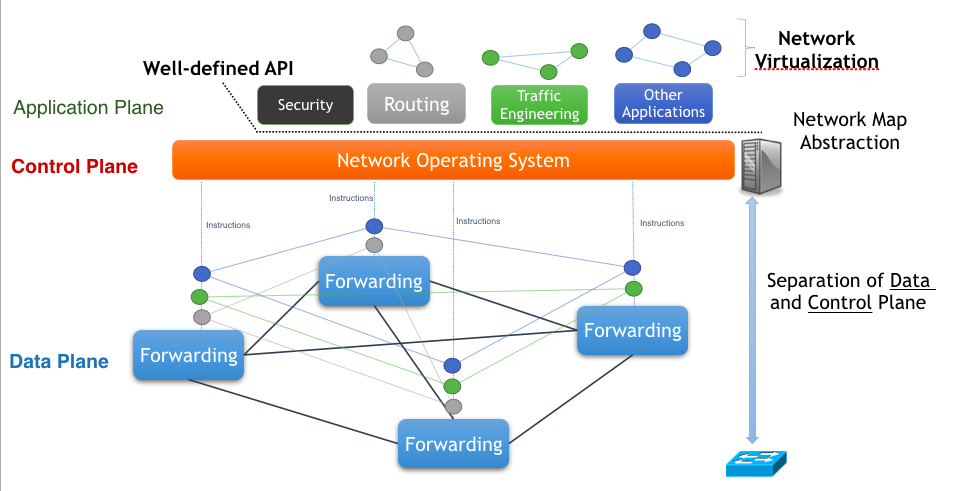
\includegraphics[scale=0.4]{data_control_plane} 
\caption{Separation of data and control planes }
\label{fig:data_control_plane}
\end{center}
\end{figure}

\subsection{Data and Control planes}
SDN consists of two separate planes which are data plane and control plane. In the traditional network where the forwarding logic is distributed to in the network. One example of this type of distribution is in the linked state routers where routers exchange information with each other to jointly create and image of the network while none of them have the complete view of the network. Unlike the traditional network, in SDN, the network intelligence is and states are logically abstracted out. The underlying network infrastructure is abstracted out from applications.
\begin{itemize}
    \item Data plane: The forwarding logic like switches run of general purpose commodity hardware. It is decoupled from specific networking hardware
    \item Control plane: The data plane is controlled, maintained and programmed from a central entity called a control plane 
\end{itemize}

\begin{figure}[h]
\begin{center}	
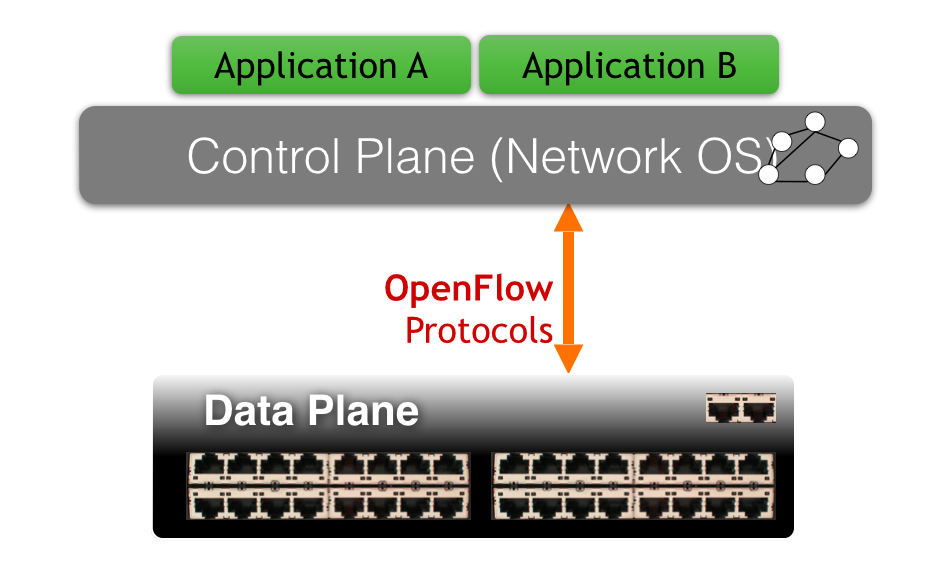
\includegraphics[scale=0.4]{openflow} 
\caption{OpenFlow}
\label{fig:openflow}
\end{center}
\end{figure}

\subsection{OpenFlow}
OpenFlow is a software defined networking standard.It allows network programmers to determine the path of network packets through a network of switches. It is a communication interface between the control plane and data plane of an SDN architecture. It allows direct access to as well as manipulation of the forwarding plane of network devices such as switches, routers, both physical and virtual. It can also be thought as a protocol for switches and controller interfaces.

\subsubsection{Working of OpenFlow}
OpenFlow manages the traffic (network flows) by manipulating a flow table at switches. Instructions are stored in flow tables. When a packet arrives at a switch, it matches the header fields with flow entries in a flow table. If any entry is matched, it performs indicated actions and updates the counters. If, however, it is not matches then the switch asks the controller by sending a message with the packet header.

% \subsubsection{OpenFlow table}
% The basic actions in an OpenFlow table are as follows:
% \begin{itemize}
%     \item All: To all interfaces except the incoming interface.
%     \item Controller: Encapsulate the packet and send it to the controller.
%     \item Local: Send to its local networking stack
%     \item Table: Perform actions in the next flow table 
%     \item In\_port: Send the packet back to the input port.
%     \item Normal: Forward in accordance with the traditional ethernet.
%     \item Flood: Send along the minimum spanning tree except the incoming interface.
% \end{itemize}

\subsection{SDN Controller}
SDN controller is a software which communicated to the hardware switches using the above mentioned OpenFlow protocols. A controller creates rules as to how a packet must be forwarded and installs these rules in hardware switches. A switch then simply forwards the packets according to the rules set up by the controller.

Now we briefly give a description of different SDN controller that are available today.

\subsubsection{Nox}
Nox was the first SDN controller that was developed. It is a C++ based controller and many other controller like pox have been developed over it. It is not in development now.

\subsubsection{Pox}
Pox is developed over Nox controller. It is a simple to use python based controller which can be used for rapid protyping of any SDN application.

\subsubsection{Ryu}
Ryu is a component based SDN framework with a well defined API. It supports various protocols other that OpenFLow like Netconf, OF-config.

\subsubsection{OpenDaylight}
OpenDaylight is an open source Java based project under Linux distribution. It has a huge community and contributors to its code base. Although a bit difficult to learn, it has a wide variety of features and is also used for commercial products.

\subsubsection{Floodlight}
Floodlight is also a Java based controller that we have used for developing our application. It has a growing community of developers and provides a rich set of northbound and southbound APIs to create an application module. 

\section{Baadal: IIT Delhi's Private Cloud}
"Baadal is a cloud orchestration and virtualization management software developed at IITD that can work with multiple virtualization technologies like KVM, Xen, and VMWare" \cite{baadaliitd}. Its main features include
\begin{itemize}
    \item Dynamic resource scheduling and power management
    \item An integrated work flow system for request of virtual machines
    \item Virtual machines can be powered on, powered off, resumed or suspended as per user requirement.
    \item Different costs for resources for VMs depending upon the requirement.
\end{itemize}

Currently Baadal is deployed in IITD on 48 blade servers with 500 cores and 50 TB of storage (which is virtualized storage based on Network attached storage or NAS). Out of these over 60 machines are being used for high performance computing in the campus.

According to \cite{baadaliitdwebpage} the technical specification of baadal are as follows:
\begin{itemize} 
    \item 32 blade servers with 2x6 core Intel(R) Xeon(R) CPU X5670 @ 2.93GHz and 16 GB RAM.
    \item 16 blade servers with 2x4 core Intel(R) Xeon(R) CPU E5540 @ 2.53GHz and 12 GB RAM.
    \item A 10Gbps ethernet backbone.
    \item 50 TB of virtualized storage on a NetApp 3210V NAS and HP EVA6400 SAN with FC disks.
    \item Open source virtualization technology based on KVM.
\end{itemize}

\subsection{Baadal sandbox}
To facilitate easy development and testing of application for use in Baadal deployment this sandbox environment is provided. It simulates the actual baadal architecture and configuration in a single machine without using any more physical hosts. Once an application is tested on this sandbox then it can be ported on the actual Baadal with little modifications.

\subsection{Netmap}
Netmap is a framework for high speed packet I/O. It is implement as a single kernel module and supports access to network cards, host stack, virtual ports and netmap pipes. 
It uses optimizations like batch processing of packets and using a circular queue as both input and output buffers. This reduces packet processing delays and eliminates copying delays.


\section{Related Work}
\subsection{SDN based Scheme for Virtual network management}
As we have seen in virtualisation services like storage, network, computing are provided using cloud. It required usage of virtual network. As part of this project, we suggested some of the changes in virtual network management schemes. But before moving onto the changes suggested and implemented we should have an idea of management schemes for the virtual network.
\begin{itemize}
    \item Three important aspects of management scheme are how to transfer virtual network packets, tenant isolation and adaptability of virtual network to topology changes.
    \item Considering these three factors management scheme can be divided into two types. One is \textbf{traditional bridging} which binds VMs NIC with physical NIC on a virtual bridge and transfer VMs packets via the physical NICs. This has advantage of good performance but it lacks flexibility.
    The other type based on \textbf{overlay network} which encapsulates the virtual network packets into the hosts packets. It has advantage of flexibility but it leads to performance loss.
    \item Using above two traditional methods we have to make a trade off between flexible management and network performance. But SDN allows us to accomplish management logic conveniently which helps to  achieve both flexibility and performance improvement.
    \item We have designed management scheme for vlan solution inspired from a scheme known as FENet.\cite{liu2014fenet}. FENet is SDN based approach for management scheme, creates virtual network upon devices which support OpenFlow protocol and SDN controller programs are developed to manage them.
    \item It provides improved network utilisation and lower latency than the scheme based on traditional bridging.
    \item Nicira Network virtualisation platform (NVP) provides a solution which combines idea of SDN and IP tunnelling. One of the other solution proposed for tenant isolation based on SDN, is conditional on the fact that hosts are in the layer 2 network.\cite{nunes2013virtualized}. It replaces the packet destination destination MAC address with the host MAC address while the destination IP address is still the VM's so that the packet routing does not happen across the physical network.
\end{itemize}

\subsection{Online traffic aware virtual machine placement in data center networks}
Dias et. al.\cite{dias2012online} have presented a virtual machine placement (VMP) algorithm to reallocate virtual machines in the data center servers based on the current traffic matrix, CPU, and memory usage. VMP takes into account the current data center work load, CPU and memory usage of virtual machines to avoid bottlenecks. The basic idea is to consolidate virtual machines that have correlated services. VMP operation is divided into four parts:

\begin{itemize}
    \item Data acquisition: The traffic between each pair of virtual machines is used to create a traffic matrix. It also takes the CPU and memory usage of each virtual machine as input as well as the topology of the data center. The most used topologies used are similar as all of them have a core which is responsible for connecting big segments of the network. Traffic engineering tries to push the traffic to the edges of the network thereby reducing it in the higher layers. 
    \item Server partitioning: They also have proposed an algorithm for partitioning of servers. The servers which have high degree of connectivity are clubbed together. Most suitable candidates for this type of aggregation are the servers which are placed at the same layers.
    \item Clustering virtual machines: They \cite{dias2012online} have used a community finding algorithm to find communities withing the virtual machines which clusters the virtual machines into groups which have high degree of connectivity.
    \item VM assignment: In the final step the virtual machines (which are clustered into communities by now) are allocated server partitions which were obtained in the server partitioning step.
\end{itemize}
In the simulations they have shown that their method is scalable to big data centers and provides an improvement of 12.5\% over no management.

\subsection{Traffic Engineering}
Jiang et. al. \cite{jiang2012joint} have proposed a solution to the problem of network load balancing by means of a joint tenant placement and route selection by exploiting multipath routing capability and dynamic virtual machine migration. They have proposed an offline algorithm that solves a static problem given a network snapshot, and an online solution for a dynamic environment with changing traffic. They have leveraged the technique of Markov approximation what required a very small number of virtual machine migrations. In simulations done by them they have evaluated the performance of online algorithms with real workload obtained from large computing clusters and have shown that their algorithm incurs the minimum performance cost in comparison to all other tested algorithms.

Biran et. al. \cite{biran2012stable} have also studied this problem and said that VM placement should consider the aggregate resource consumption of co-located VMs in order to obey service level agreements at lower possible cost. Also, the traffic patterns are not stable in nature and vary over a period of time. They have addressed this problem by trying to allocate a placement that not only satisfies the predicted communication demand but also is resilient to demand time-variations. They have defined the problem as a min cut ratio-aware VM placement which is NP-hard in general but they have employed several heuristics to solve it. Through their simulations they have shown that the placements based on their algorithm increase data scalability, while being able to support time-varying traffic demands with a reduced number of dropped packets. 

\subsection{Network Function Virtualization}
Middleboxes like proxy servers, firewall, NAT, etc. have become indispensable for today's networks. However, they come with problems like being expensive, difficult to manage and scale. Many of these problems arise because of the fact that they are hardware based devices. As a solution to this problem a recent trend toward Network Function Virtualization has started to turn these middleboxes into software-based entities.

Matins et. al. \cite{martins2014clickos} have introduced a virtualized software middlebox platform called ClickOS. It is based on Xen sice it provides para-virtualized VMs to build a low delay and high throughput platform. Through their evaluation they have shown that ClickOS can hundreds of middleboxes on commodity hardware, offers millions of packet per seconds processing and provide low packet delays. They have shown that even low-end servers can forward packets at 30Gbps. 

Ge et. al. \cite{ge2014openanfv} have built a consolidated framework OpenANFV for speeding up the performances of virutalized middleboxes. When a middlebox is needed its resources are orchestrated by OpenStack and is instantiated as a virtual machines on a common platform. They have a Network Functions Acceleration Platform (NFAP) which provides a FPGA card which accelerates various functions. In their evaluations they have shown orders of magnitude of improvement in throughput in virtualized middleboxes like deep  packet inspection, network address translation, etc. using NFAP as compared to without NFAP.

Han et. al. \cite{han2015network} have  explained the requirements, architectural framework and use cases for NFV and have also discussed the challenges in this area. They argue that although virtualization impacts performance negatively in terms of throughput and latency, these effect must be kept to a minimum. Migrating from the existing architecture to NFV based solution is also a major hurdle that network carriers face. They have presented a architectural framework for NFV which includes four components - orchestrator, VNF manager, virtualization layer and virtualized infrastructure manager. They have also given various use cases for NFV like virtualization of cellular base station, virtualization of cellular core network and virtualization of home network.